\immediate\write18{tex hobby.dtx}
\documentclass{ltxdoc}
\usepackage[T1]{fontenc}
\usepackage{csquotes}
\usepackage{lmodern}
\usepackage{tikz}
\usepackage{pgfplots}
\usepackage{amsmath}
\usepackage{fancyvrb}
\usetikzlibrary{hobby,decorations.pathreplacing}
\usepackage{listings}
\usepackage{hyperref}
\pgfplotsset{compat=1.9}

\lstset{
  breakatwhitespace=true,
  breaklines=true,
  language=[LaTeX]TeX,
  basicstyle=\small\ttfamily,
  keepspaces=true,
  columns=fullflexible
}
% hobby specific keywords (we can't put keywords with spaces :()
\lstset{
  emphstyle={\color{red}},
  emph={and,angle,blank,blanks,closed,controls,curl,curve,designated,disjoint,excess,finish,Hobby,hobby,in,invert,next,out,path,previous,quick,restore,save,shortcut,show,soft,tension,through,use}
}
% tikz keywords used in this documentation
\lstset{
  emphstyle={[2]\color{blue!70!black}},
  emph={[2]addplot,axis,blue,coordinates,distance,double,draw,every,foreach,grid,help,line,lines,plot,postaction,red,rotate,scale smooth,scale,smooth,style,thick,tikz,tikzpicture,to,ultra,white,width,xshift,yellow}
}

\EnableCrossrefs
\CodelineIndex
\RecordChanges

\newenvironment{example}
  {\VerbatimEnvironment
   \begin{VerbatimOut}{example.out}}
  {\end{VerbatimOut}
   \begin{center}
   \setlength{\parindent}{0pt}
   \fbox{\begin{minipage}{.9\linewidth}
     \lstinputlisting[]{example.out}
   \end{minipage}}
   \fbox{\begin{minipage}{.9\linewidth}
     \centering
     \input{example.out}
   \end{minipage}}
\end{center}
}



\tikzset{
  show curve controls/.style={
    decoration={
      show path construction,
      curveto code={
  \draw [blue, dashed]
        (\tikzinputsegmentfirst)    -- (\tikzinputsegmentsupporta)
        node [at end, draw, solid, red, inner sep=2pt]{};
  \draw [blue, dashed]
        (\tikzinputsegmentsupportb) -- (\tikzinputsegmentlast)
        node [at start, draw, solid, red, inner sep=2pt]{};
      }
    },decorate
  },
}

%\bibliographystyle{plain}

\renewcommand{\thefootnote}{\fnsymbol{footnote}}

\providecommand*{\url}{\texttt}
\title{The \textsf{Hobby} package}
\author{Andrew Stacey \\ \url{loopspace@mathforge.org}}
\date{\hobbyVersion\ from\ \hobbyDate}
\begin{document}
\maketitle

\section{Introduction}

John Hobby's algorithm, \cite{MR834054}, produces a curve through a given set of points.
The curve is constructed as a list of cubic B\'ezier curves with endpoints at subsequent points in the list.
The parameters of the curves are chosen so that the joins are ``smooth''.
The algorithm was devised as part of the MetaPost program.

TikZ/PGF has the ability to draw a curve through a given set of points but its algorithm is somewhat simpler than Hobby's and consequently does not produce as aesthetically pleasing curve as Hobby's algorithm does.
This package implements Hobby's algorithm in \TeX{} so that TikZ/PGF can make use of it and thus produce nicer curves through a given set of points.

Hobby's algorithm allows for considerable customisation in that it can take into account various parameters.
These are all allowed in this implementation.

There is also a ``quick'' version presented here.
This is a modification of Hobby's algorithm with the feature that any point only influences a finite number (in fact, two) of the previous segments (in Hobby's algorithm the influence of a point dies out exponentially but never completely).
This is achieved by applying Hobby's algorithm to subpaths.
The resulting path produced with this ``quick'' version is not as ideal as that produced by Hobby's full algorithm, but is still much better than that produced by the \Verb+plot[smooth]+ method in TikZ/PGF, as can be seen in Figure~\ref{fig:comparison}.
As this is intended as a simpler method, it does not (at present) admit the same level of customisation as the full implementation.
The ``quick'' algorithm is described in full in Section~\ref{sec:quick}.

The full algorithm is implemented in \LaTeX3 with no reference to TikZ or PGF.
It makes extensive use of the \Verb+fp+ and \Verb+prop+ libraries for the computation steps.
The TikZ library is simply a wrapper that takes the user's input, converts it into the right format for the \LaTeX3 code, and then calls that code to generate the path.
The ``quick'' version does not use \LaTeX3 and relies instead on the \Verb+PGFMath+ library for the computation.


Figure~\ref{fig:comparison} is a comparison of the three methods.
The red curve is drawn using Hobby's algorithm.
The blue curve is drawn with the \Verb+plot[smooth]+ method from TikZ/PGF.
The green curve uses the ``quick'' version.
Figure~\ref{fig:metapost} compares the implementation with that given by MetaPost.

\begin{figure}
\centering
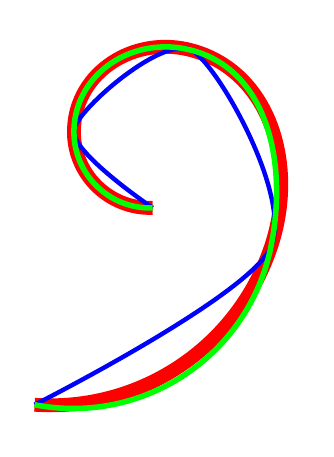
\begin{tikzpicture}[scale=.5]
\draw[red,line width=5pt] (0,0) to[curve through={(6,4) .. (4,9) .. (1,7)}] (3,5);
\draw[ultra thick,blue] plot[smooth] coordinates {(0,0) (6,4) (4,9) (1,7) (3,5)};
\draw[green,line width=2pt] (0,0) to[quick curve through={(6,4) (4,9)  (1,7)}] (3,5);
\end{tikzpicture}
\caption{Comparison of the three algorithms}
\label{fig:comparison}
\end{figure}


\begin{figure}
\centering
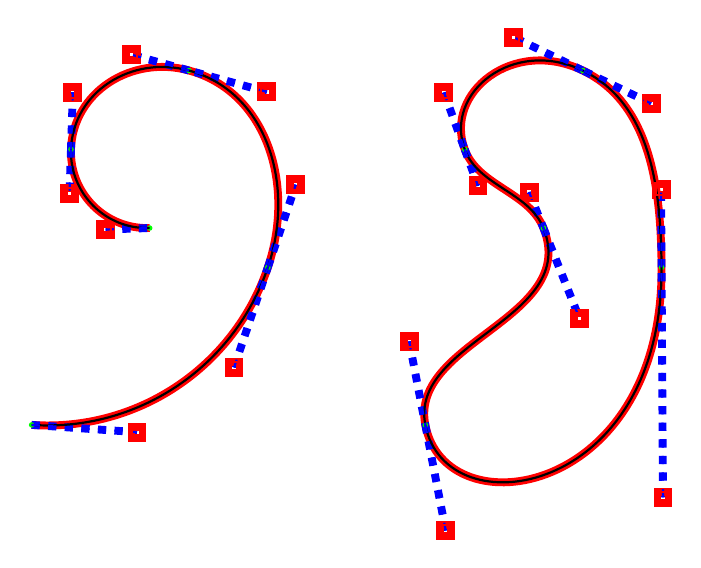
\begin{tikzpicture}[scale=.5]
  \draw[scale=.1,postaction=show curve controls,line width=1mm,red] (0,0)
    .. controls (26.76463,-1.84543) and (51.4094,14.58441) .. (60,40)
    .. controls (67.09875,61.00188) and (59.76253,84.57518) .. (40,90)
    .. controls (25.35715,94.01947) and (10.48064,84.5022) .. (10,70)
    .. controls (9.62895,58.80421) and (18.80421,49.62895) .. (30,50);
  \fill[green] (0,0) circle[radius=2pt]
    (6,4) circle[radius=2pt]
    (4,9) circle[radius=2pt]
    (1,7) circle[radius=2pt]
    (3,5) circle[radius=2pt];
  \draw[postaction=show curve controls,thick] (0,0) to[curve through={(6,4) .. (4,9) .. (1,7)}] (3,5);
  \begin{scope}[xshift=10cm]
    \draw[scale=.1,postaction=show curve controls,line width=1mm,red] (0,0)
      .. controls (5.18756,-26.8353) and (60.36073,-18.40036) .. (60,40)
      .. controls (59.87714,59.889) and (57.33896,81.64203) .. (40,90)
      .. controls (22.39987,98.48387) and (4.72404,84.46368) .. (10,70)
      .. controls (13.38637,60.7165) and (26.35591,59.1351) .. (30,50)
      .. controls (39.19409,26.95198) and (-4.10555,21.23804) .. (0,0); %
    \fill[green] (0,0) circle[radius=2pt]
      (6,4) circle[radius=2pt]
      (4,9) circle[radius=2pt]
      (1,7) circle[radius=2pt]
      (3,5) circle[radius=2pt];
    \draw[postaction=show curve controls,thick] (0,0) to[closed,curve through={(6,4) .. (4,9) .. (1,7)}] (3,5);
  \end{scope}
\end{tikzpicture}
\caption{Hobby's algorithm in TikZ overlaying the output of MetaPost}
\label{fig:metapost}
\end{figure}

\section{Usage}
The package is provided in form of a TikZ library.
It can be loaded with
\begin{verbatim}
\usetikzlibrary{hobby}
\end{verbatim}

\textbf{Warning}: This package makes extensive use of \LaTeX3.
On occasion, updates to \LaTeX3 packages have resulted in this package behaving oddly or not working at all.
The most up to date version of this package can be obtained from my \href{https://github.org/loopspace/hobby}{github page} (download \Verb+hobby.dtx+ and run \Verb+tex hobby.dtx+ to generate the files).
Often, such issues are reported on the \href{http://tex.stackexchange.com}{TeX-SX} site and workarounds quickly found so it is worth checking there as well.

\bigskip

There are a variety of ways of specifying the data to the algorithm to generate the curve.

\subsection{As a \textsf{to path}.}

The key \Verb+curve through={<points>}+ installs a \Verb+to path+ which draws a smooth curve through the given points.
The points should be specified as a list which can be optionally separated by dots.
The purpose of allowing the dots is to make it simpler to switch between the \Verb+to path+ method and the \Verb+shortcut+ method (described in Section~\ref{sec:shortcut}).
However, note that the two methods are not completely synonymous due to how one can specify options so care must still be taken when switching.

\begin{example}
\begin{tikzpicture}[scale=.5]
  \draw (0,0) to[curve through={(6,4) .. (4,9) .. (1,7)}] (3,5);
\end{tikzpicture}
\end{example}

\begin{example}
\begin{tikzpicture}[scale=.5]
  \draw (0,0) to[curve through={(6,4) (4,9) (1,7)}] (3,5);
\end{tikzpicture}
\end{example}

There is a corresponding key \Verb+quick curve through={<points>}+ which uses the ``quick'' algorithm.
Again, the dots are optional.

\begin{example}
\begin{tikzpicture}[scale=.5]
  \draw (0,0) to[quick curve through={(6,4) .. (4,9) .. (1,7)}] (3,5);
\end{tikzpicture}
\end{example}

\subsection{The \textsf{shortcut} Method}
\label{sec:shortcut}

There is also the facility to subvert TikZ's path processor and define curves simply using the \Verb+..+ separator between points.
Note that this relies on something a little special in TikZ: the syntax \Verb+(0,0) .. (2,3)+ is currently detected and processed but there is no action assigned to that syntax.
As a later version of TikZ may assign some action to that syntax, this package makes its override optional via the key \Verb+use Hobby shortcut+ (which can be set globally if so desired).

\begin{example}
\begin{tikzpicture}[scale=.5,use Hobby shortcut]
  \draw (-3,0) -- (0,0) .. (6,4) .. (4,9) .. (1,7) .. (3,5) -- ++(2,0);
\end{tikzpicture}
\end{example}

\begin{example}
\begin{tikzpicture}[scale=.5,use quick Hobby shortcut]
  \draw (-3,0) -- (0,0) .. (6,4) .. (4,9) .. (1,7) .. (3,5) -- ++(2,0);
\end{tikzpicture}
\end{example}

\subsection{The \textsf{Plot Handler} Method}

The algorithms can also be used via the \Verb+plot handler+ syntax.
This library registers three plot handlers: \Verb+hobby+, \Verb+closed hobby+, and \Verb+quick hobby+.
The first is an open curve through the points using the full algorithm, the second is a closed curve, and the third uses the quick algorithm (and is thus an open curve).

\begin{example}
  \tikz[smooth] \draw plot coordinates {(0,0) (1,1) (2,0) (3,1) (2,1) (10:2cm)};

  \tikz[hobby] \draw plot coordinates {(0,0) (1,1) (2,0) (3,1) (2,1) (10:2cm)};

  \tikz[closed hobby] \draw plot coordinates {(0,0) (1,1) (2,0) (3,1) (2,1) (10:2cm)};

  \tikz[quick hobby] \draw plot coordinates {(0,0) (1,1) (2,0) (3,1) (2,1) (10:2cm)};
\end{example}

This has the side effect that these can be used with the \Verb+pgfplots+ package.
However, the Hobby algorithm is designed to draw a curve in 2D-{}space and does not take into account the fact that when plotting a graph then the two dimensions are treated differently.

\begin{example}
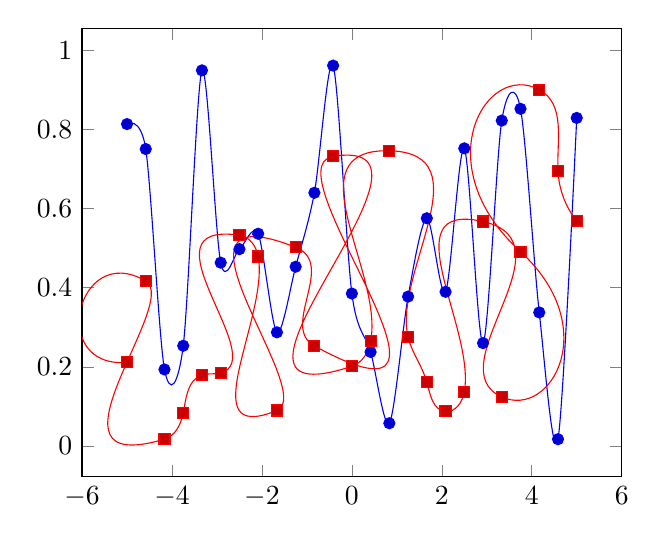
\begin{tikzpicture}
  \begin{axis}
    \addplot +[smooth] {rnd};
    \addplot +[hobby] {rnd};
  \end{axis}
\end{tikzpicture}
\end{example}

\subsection{Basic Level PGF Commands}

(Suggested by the question \href{http://tex.stackexchange.com/q/159896/86}{How to combine Hobby paths with PGF Basic Layer commands?} on TeX-SX.)

In some circumstances, it is convenient to bypass TikZ and use more basic PGF commands for building a path.
It is possible to add a path built using Hobby's algorithm in this fashion.
The commands are:

\begin{itemize}
\item \Verb+\pgfpathhobby+ to initialise the path.
If this is followed by a braced group then the contents of that are taken as options to the algorithm.

\item \Verb+\pgfpathhobbypt{<pgf point specification>}+ to add a point to the path.
If this is followed by a braced group then the contents of that are taken as options for that point.

\item \Verb+\pgfpathhobbyend+ finalises the path.
This applies the algorithm to the set of specified points and adds it to the current path.
\end{itemize}

\begin{example}
\begin{tikzpicture}
  \pgfpathmoveto{\pgfpoint{0}{0}}
  \pgfpathlineto{\pgfpoint{1cm}{0}}
  \pgfpathhobby{closed=true}
  \pgfpathhobbypt{\pgfpoint{1cm}{2cm}}{tension in=2}
  \pgfpathhobbypt{\pgfpoint{2cm}{1cm}}
  \pgfpathhobbypt{\pgfpoint{3cm}{0cm}}
  \pgfpathhobbyend
  \pgfusepath{stroke}
\end{tikzpicture}
\end{example}

\section{Customisation}

There are various ways to customise the path generated by the Hobby algorithms.
The full algorithm has a variety of parameters which can be varied to produce different paths through the same points.
These vary from specifying that the path be open or closed, to specifying ``tensions'' at each point to change how the path approaches or leaves it.

\subsection{Algorithm Customisations}

The main algorithm (i.e., not the ``quick'' variant) can deal with open or closed paths, it is possible to vary the ``tensions'' between the specified points of the paths, and for an open path it is possible to specify the incoming and outgoing angles either directly or via certain ``curl'' parameters.
When using the \Verb+to path+ specification, the parameters can be specified before or after the \Verb+curve through+ key or as options to the coordinates.
When using the \Verb+shortcut+ specification, the parameters can be given on the path or on coordinates.

On occasion, it is ambiguous which curve an option belongs to.
This is most likely if a coordinate happens to belong to two curves, or if a coordinate is parsed before TikZ knows that it is constructing a curve using this library.
The simplest solution is to move the option to a place where there is no ambiguity.
Other solutions to this problem will be detailed later.

Let us start with the customisations to the algorithm.

\begin{itemize}
\item Basic curve.
\begin{example}
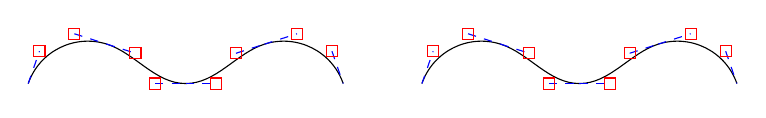
\begin{tikzpicture}
  \draw[postaction=show curve controls] (0,0) to[curve through={(1,.5) .. (2,0) .. (3,.5)}] (4,0);
  \draw[xshift=5cm,use Hobby shortcut,postaction=show curve controls] (0,0) .. (1,.5) .. (2,0) .. (3,.5) .. (4,0);
\end{tikzpicture}
\end{example}

\item The path can be open, as above, or closed.
%%
\begin{example}
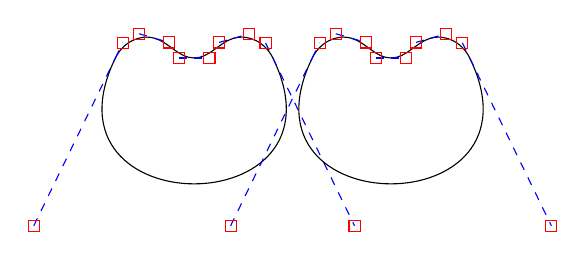
\begin{tikzpicture}[scale=.5]
  \draw[postaction=show curve controls] (0,0) to[closed,curve through={(1,.5) .. (2,0) .. (3,.5)}] (4,0);
  \draw[xshift=5cm,use Hobby shortcut,postaction=show curve controls] ([closed]0,0) .. (1,.5) .. (2,0) .. (3,.5) .. (4,0);
\end{tikzpicture}
\end{example}

\item Specifying the angle at which the curve goes \emph{out} and at which it comes \emph{in}.
The angles given are absolute.
\begin{example}
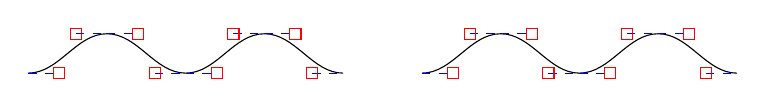
\begin{tikzpicture}
  \draw[postaction=show curve controls] (0,0) to[out angle=0,in angle=180,curve through={(1,.5) .. (2,0) .. (3,.5)}] (4,0);
  \draw[xshift=5cm,use Hobby shortcut,postaction=show curve controls] ([out angle=0,in angle=180]0,0) .. (1,.5) .. (2,0) .. (3,.5) .. (4,0);
\end{tikzpicture}
\end{example}

\item Applying tension as the curve comes in to a point.
\begin{example}
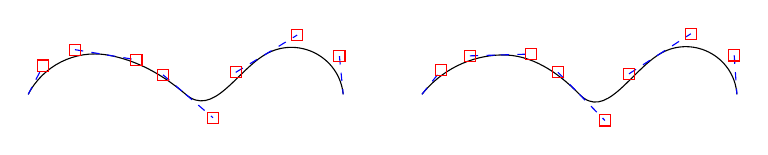
\begin{tikzpicture}
  \draw[postaction=show curve controls] (0,0) to[curve through={(1,.5) .. ([tension in=2]2,0) .. (3,.5)}] (4,0);
  \draw[xshift=5cm,use Hobby shortcut,postaction=show curve controls] (0,0) .. (1,.5) .. ([tension in=2]2,0) .. (3,.5) .. (4,0);
\end{tikzpicture}
\end{example}

\item Applying the same tension as a curve comes in and goes out of a point.
\begin{example}
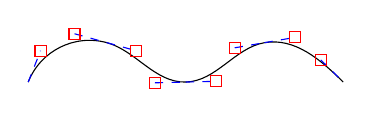
\begin{tikzpicture}
  \draw[postaction=show curve controls] (0,0) to[curve through={(1,.5) .. ([tension=2]2,0) .. (3,.5)}] (4,0);
\end{tikzpicture}
\end{example}

\item Specifying the \emph{curl} parameters.
\begin{example}
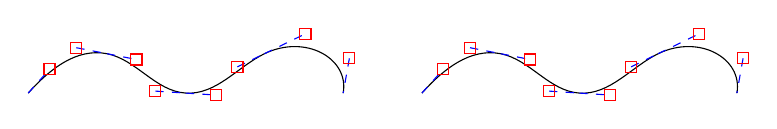
\begin{tikzpicture}
  \draw[postaction=show curve controls] (0,0) to[in curl=.1,out curl=3,curve through={(1,.5) .. (2,0) .. (3,.5)}] (4,0);
  \draw[xshift=5cm,use Hobby shortcut,postaction=show curve controls] (0,0) .. ([in curl=.1,out curl=3]1,.5) .. (2,0) .. (3,.5) .. (4,0);
\end{tikzpicture}
\end{example}
\end{itemize}

\subsection{Edge Cases}

Angles are constrained to lie in the interval \((-\pi,\pi]\).
This can introduce edge cases as there is a point where we have to compare an angle with \(-\pi\) and if it is equal, add \(2 \pi\).
This will occur if the path ``doubles back'' on itself as in the next example.
By nudging the repeated point slightly, the behaviour changes drastically.

\begin{example}
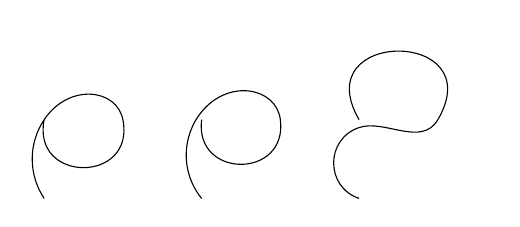
\begin{tikzpicture}[use Hobby shortcut]
  \draw (0,0) .. (1,0) .. (0,0) .. (0,-1);
  \draw[xshift=2cm] (0,0) .. (1,0) .. (0,0.1) .. (0,-1);
  \draw[xshift=4cm] (0,0) .. (1,0) .. (0,-0.1) .. (0,-1);
\end{tikzpicture}
\end{example}

Due to the precision of the computations, it is not possible to always get this test correct.
The simplest solution is to nudge the repeated point in one direction or the other.
Experimenting shows that the ``nudge factor'' can be extremely small (note that it will be proportional to the distance between the specified points).
It is best to nudge it in the direction most normal to the line between the specified points as the goal is to nudge the difference of the angles.
An alternative solution is to add an additional point for the curve to go through.
\begin{example}
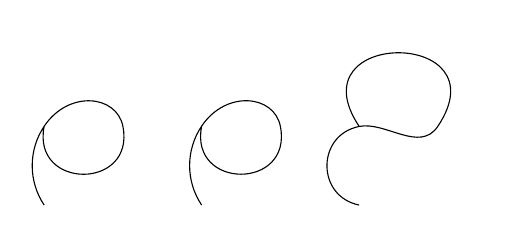
\begin{tikzpicture}[use Hobby shortcut]
  \draw (0,0) .. (1,0) .. (0,0) .. (0,-1);
  \draw[xshift=2cm] (0,0) .. (1,0) .. (0,0.002) .. (0,-1);
  \draw[xshift=4cm] (0,0) .. (1,0) .. (0,-0.002) .. (0,-1);
\end{tikzpicture}
\end{example}

Lastly, it is possible to add an \Verb+excess angle+ key to a coordinate.
This will add the corresponding multiple of \(2\pi\) to the angle difference.
\begin{example}
\begin{tikzpicture}[use Hobby shortcut]
  \draw (0,0) .. (1,0) .. (0,0) .. (0,-1);
  \draw[xshift=2cm] (0,0) .. ([excess angle=1]1,0) .. (0,0) .. (0,-1);
  \draw[xshift=4cm] (0,0) .. ([excess angle=-1]1,0) .. (0,0) .. (0,-1);
\end{tikzpicture}
\end{example}

Although this is intended to be an integer, no check is done and so some quite odd curves can result from changing this parameter.

\subsection{Reusing Paths}

Although the (full) algorithm has good theoretical computation time, using \TeX\ for its implementation does not provide for fast runs.
The externalisation library of TikZ/PGF can be used to save whole pictures, but it can be useful to save a generated path within a single \Verb+tikzpicture+ for later use within that same picture.
The implementation allows for this by separating the generation of the path from its use.

\begin{example}
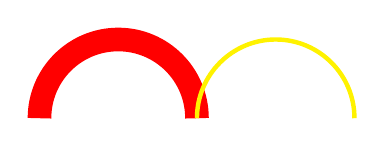
\begin{tikzpicture}
  \draw[line width=3mm,red,use Hobby shortcut,save Hobby path={saved}] (0,0) .. (1,1) .. (2,0);
  \draw[xshift=2cm,ultra thick,yellow] (0,0) [restore and use Hobby path={saved}{}];
\end{tikzpicture}
\end{example}
%

Note that the key \Verb+restore and use Hobby path+ is given \emph{after} the initial \Verb+(0,0)+.
This is because by default the path generated by the Hobby algorithm does not start with an explicit \Verb+moveto+ since that is the standard behaviour of all of PGF's path construction macros.
So the \Verb+(0,0)+ ensures that our path is well-{}formed by issuing an initial \Verb+moveto+.
An alternative would be to use the key \Verb+disjoint+ which does add an initial \Verb+moveto+.

\begin{example}
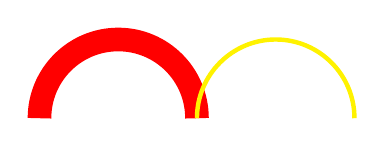
\begin{tikzpicture}
  \draw[line width=3mm,red,use Hobby shortcut,save Hobby path={saved}] (0,0) .. (1,1) .. (2,0);
  \draw[xshift=2cm,ultra thick,yellow,restore and use Hobby path={saved}{disjoint}];
\end{tikzpicture}
\end{example}
%

An example of where this is useful is in drawing knot diagrams.
When so doing, it is sometimes convenient to draw a path (or segment of a path) twice in order to get the under/over crossings correct.
For this situation, it can be useful to designate certain parts of the path as \Verb+blank+, whereby we mean to redraw them later.
The point of a blank segment of a curve is that it is still taken into account when computing the algorithm but is left blank when it comes to rendering.
A path can then be redrawn with the blank/non-{}blank segments reversed.
As it might be desired to have only some blank segments drawn the second time, there are two types of blank.
Only a \Verb+soft+ blank will be reversed in these circumstances.

\begin{example}
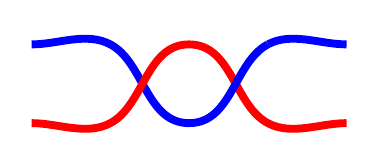
\begin{tikzpicture}[use Hobby shortcut,line width=1mm,rotate=90]
  \draw[blue,save Hobby path={left}] ([out angle=90,in angle=-90]1,0) .. (1,1) .. ([blank=soft]0,2) .. (1,3) .. (1,4);
  \draw[red] ([out angle=90,in angle=-90]0,0) .. (0,1) .. (1,2) .. (0,3) .. (0,4);
  \draw[blue,restore and use Hobby path={left}{disjoint,invert soft blanks}];
\end{tikzpicture}
\end{example}
%

This can be taken a step further.
The generated data can be saved to the \Verb+aux+ file and read back in, avoiding the need to regenerate it on each run.
To engage this facility, the Hobby path has to be named (via \Verb+save Hobby path+) and the key \Verb+Hobby externalise+ (or \Verb+Hobby externalize+) must be given in a context that applies (such as on the path or on the surrounding scope).

\bigskip


The relevant keys are the following.

\begin{itemize}
\item \Verb+use previous Hobby path[=<options>]+.
This (re)uses the previously generated Hobby path.
As all the data is globally stored, this can technically be in a different \Verb+tikzpicture+.
The \Verb+<options>+ will be applied, in so far as they are options that can be applied after the algorithm has run.

\item \Verb+save Hobby path=<name>+.
Saves a path for later use.
The path is saved in a global macro so can be reused in another picture.

\item \Verb+restore Hobby path=<name>+.
This restores the named Hobby path (if it exists).
It does not \emph{use} it.
After this key, \Verb+use previous Hobby path+ will use the restored path.

\item \Verb+restore and use Hobby path={<name>}{<options>}+.
This restores the named path and uses it with \Verb+<options>+ applied.

\item \Verb+Hobby externalise+ or \Verb+Hobby externalize+.
This puts in place the code for saving the generated data to the \Verb+aux+ file.
On subsequent runs, it uses the saved data rather than the current data.
For a curve to make use of this, it has to be named via the \Verb+save Hobby path+ key.
So to regenerate the data, either delete the \Verb+aux+ file, remove the \Verb+save Hobby path+ key for one compilation run, or issue the command \Verb+\HobbyDisableAux+ which disables writing paths to the \Verb+aux+ file (note that the paths will be regenerated on the run \emph{after} the first run with this command issued).
\end{itemize}

The options that can be applied are those that affect the rendering of the curve but not its generation.
When the curve is rendered (or \emph{used}, in the above parlance), \TeX\ steps along the coordinates of the generated curve and carries out an action for each piece.
This action can be modified after the curve has been generated.
The action will be one of:
%
\begin{itemize}
\item Move to the end point (ignoring the control points).
\item Draw a Bezier curve to the end point through the control points.
\item Draw a Bezier curve to the end point through the control points and then move to the end point.
\end{itemize}
%
The last is subtle: the move doesn't actually go anywhere but it ``breaks'' the curve at the designated point.
In particular, a later \Verb+cycle+ would return to this point (or a later break) rather than to the start of the curve.

These actions are triggered by the keys \Verb+blank+ and \Verb+break+.
Each should be specified to the coordinate at the \emph{end} of the segment under consideration.
The \Verb+blank+ key can be given the argument \Verb+soft+.
The effect of this is seen when the key \Verb+invert soft blanks+ is used.
This swaps the drawing action so that non-{}blank segments are skipped and \emph{soft} blanks are drawn.
Non-{}soft-{}blank segments are still not drawn.

\begin{example}
\begin{tikzpicture}[use Hobby shortcut]
  \draw (0,0) .. (1,1) .. ([blank=soft]2,0) .. (3,1) .. ([blank]4,0) .. (5,1);
  \draw[red,use previous Hobby path={invert soft blanks,disjoint}];
\end{tikzpicture}
\end{example}
%

As a more practical application, consider the following rendering of a trefoil knot.

\begin{example}
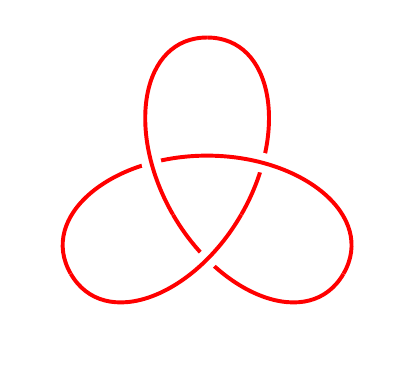
\begin{tikzpicture}[
  use Hobby shortcut,
  every path/.style={
    line width=1mm,
    white,
    double=red,
    double distance=.5mm
  }
]
  \draw ([closed]0,2) .. ([blank=soft]210:.5) .. (-30:2) .. ([blank=soft]0,.5) .. (210:2) .. ([blank=soft]-30:.5);
  \draw[use previous Hobby path={invert soft blanks,disjoint}];
\end{tikzpicture}
\end{example}
%

This could easily be generalised using the \Verb+\foreach+ command, as demonstrated in the next code.

\begin{example}
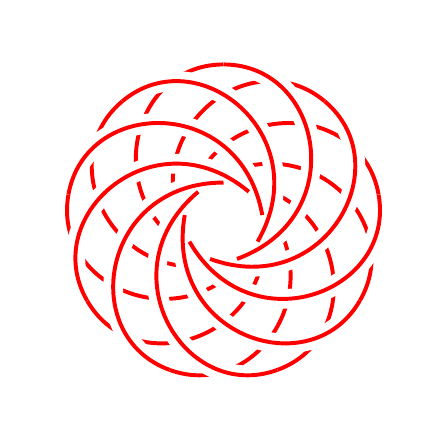
\begin{tikzpicture}[
  use Hobby shortcut,
  every path/.style={
    line width=1mm,
    white,
    double=red,
    double distance=.5mm
  }
]
\def\nfoil{9}
  \draw ([closed]0,2)
    foreach \k in {1,...,\nfoil}{
      .. ([blank=soft]90+360*\k/\nfoil-180/\nfoil:-.5) .. (90+360*\k/\nfoil:2)
    };
  \draw[use previous Hobby path={invert soft blanks,disjoint}];
\end{tikzpicture}
\end{example}
%

\subsection{Breaking the Path}

One issue with the shortcut notation is that it is not possible (using this notation) to have two sets of curves following directly on from each other because there is no clear demarcation of the boundary.
To make this possible, there is a key \Verb+Hobby action+, which installs an action to be taken after the point has been processed.
The general key \Verb+Hobby action={code}+ can install arbitrary code.
Probably the more useful variant is \Verb+Hobby finish+ which runs the algorithm on the points gathered so far.
An example of the use of this is to make it possible to specify tangencies at certain points.
Technically, once a tangent direction has been specified, the Hobby algorithm splits the set of points there and works on each piece separately.
The following key implements this, the technicalities are due to the fact that the tangent angle has to be used twice: once to specify the angle of the path coming in to that point and once to specify the angle of the path coming out.
Note that specifying the tangent vector at every point means that the algorithm is not actually being used.
However, Hobby's formulae for the lengths of the control points is still being used.

\begin{example}
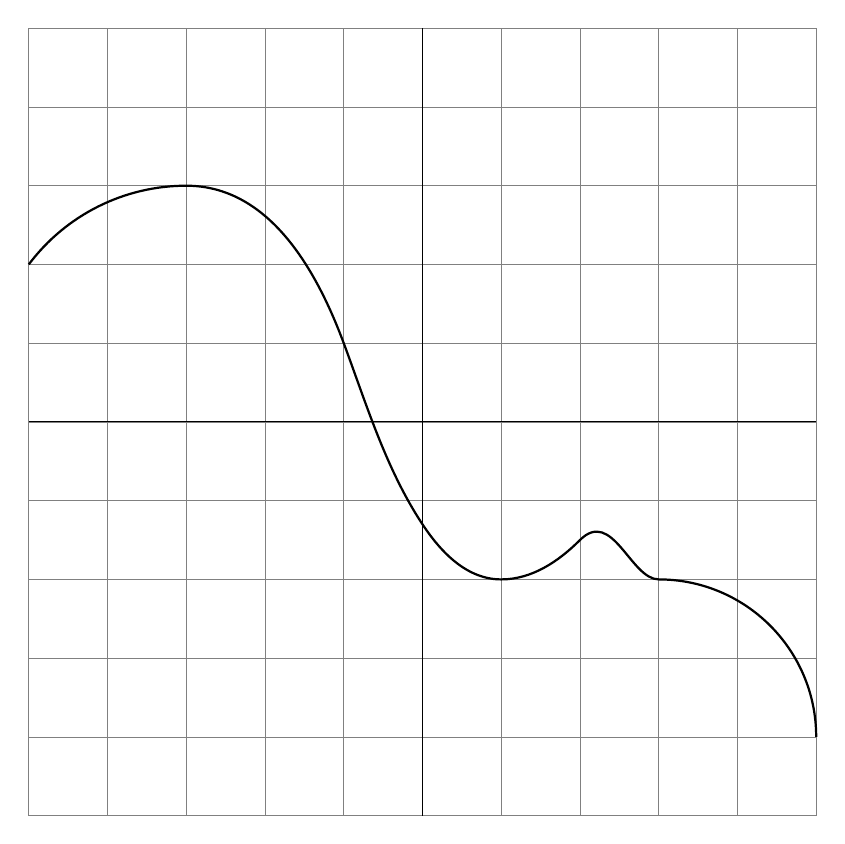
\begin{tikzpicture}[
  use Hobby shortcut,
  tangent/.style={%
    in angle={(180+#1)},
    Hobby finish,
    designated Hobby path=next,
    out angle=#1,
  },
]
  \draw[help lines] (-5,-5) grid (5,5);
  \draw (-5,0) -- (5,0) (0,-5) -- (0,5);
  \draw[thick] (-5,2) .. ([tangent=0]-3,3) .. (-1,1) .. (0,-1.3) .. ([tangent=0]1,-2) .. ([tangent=45]2,-1.5) .. ([tangent=0]3,-2) .. (5,-4);
\end{tikzpicture}
\end{example}
%



\section{Implementing Hobby's Algorithm}
We start with a list of \(n+1\) points, \(z_0, \dotsc, z_n\).
The base code assumes that these are already stored in two arrays\footnote{Arrays are thinly disguised property lists.}: the \(x\)--coordinates in \Verb+\l_hobby_points_x_array+ and the \(y\)--coordinates in \Verb+\l_hobby_points_y_array+.
As our arrays are \(0\)--indexed, the actual number of points is one more than this.
For a closed curve, we have \(z_n = z_0\)\footnote{Note that there is a difference between a closed curve and an open curve whose endpoints happen to overlap.}.
For closed curves it will be convenient to add an additional point at \(z_1\): thus \(z_{n+1} = z_1\).
This makes \(z_n\) an internal point and makes the algorithms for closed paths and open paths agree longer than they would otherwise.
The number of apparent points is stored as \Verb+\l_hobby_npoints_int+.
Thus for an open path, \Verb+\l_hobby_npoints_int+ is \(n\), whilst for a closed path, it is \(n+1\)\footnote{In fact, we allow for the case where the user specifies a closed path but with \(z_n \ne z_0\).
In that case, we assume that the user meant to repeat \(z_0\).
This adds another point to the list.}.
Following Hobby, let us write \(n'\) for \(n\) if the path is open and \(n+1\) if closed.
From this we compute the distances and angles between successive points, storing these again as arrays.
These are \Verb+\l_hobby_distances_array+ and \Verb+\l_hobby_angles_array+.
The term indexed by \(k\) is the distance (or angle) of the line between the \(k\)th point and the \(k+1\)th point.
For the internal nodes\footnote{Hobby calls the specified points \emph{knots}.}, we store the difference in the angles in \Verb+\l_hobby_psi_array+.
The \(k\)th value on this is the angle subtended at the \(k\)th node.
This is thus indexed from \(1\) to \(n'-1\).
The bulk of the work consists in setting up a linear system to compute the angles of the control points.
At a node, say \(z_i\), we have various pieces of information:
\begin{enumerate}
\item The angle of the incoming curve, \(\phi_i\), relative to the straight line from \(z_{i-1}\) to \(z_i\)
\item The angle of the outgoing curve, \(\theta_i\), relative to the straight line from \(z_i\) to \(z_{i+1}\)
\item The tension of the incoming curve, \(\overline{\tau}_i\)
\item The tension of the outgoing curve, \(\tau_i\)
\item The speed of the incoming curve, \(\sigma_i\)
\item The speed of the outgoing curve, \(\rho_i\)
\end{enumerate}
The tensions are known at the start.
The speeds are computed from the angles.
Thus the key thing to compute is the angles.
This is done by imposing a ``mock curvature'' condition.
The formula for the mock curvature is:
%%
\[
\hat{k}(\theta,\phi,\tau,\overline{\tau}) = \tau^2 \left( \frac{2(\theta + \phi)}{\overline{\tau}} - 6\theta\right)
\]
%%
and the condition that the mock curvatures have to satisfy is that at each \emph{internal} node, the curvatures must match:
%
\[
\hat{k}(\phi_i,\theta_{i-1},\overline{\tau}_i,\tau_{i-1})/d_{i-1} = \hat{k}(\theta_i,\phi_{i+1},\tau_i,\overline{\tau}_{i+1})/d_i.
\]
%%
Substituting in yields:
%%
\[
\frac{\overline{\tau}_i^2}{d_{i-1}} \left( \frac{2(\phi_i + \theta_{i-1})}{\tau_{i-1}} - 6\phi_i\right) = \frac{\tau_i^2}{d_i} \left( \frac{2(\theta_i + \phi_{i+1})}{\overline{\tau}_{i+1}} - 6\theta_i \right).
\]
%%
Let us rearrange that to the following:
%%
\begin{align*}
d_i \overline{\tau}_{i+1} \overline{\tau}_i^2 &\theta_{i-1} \\
%%
{}+
d_i \overline{\tau}_{i+1} \overline{\tau}_i^2 (1 - 3 \tau_{i-1}) &\phi_i \\
%%
{}-
d_{i-1} \tau_{i-1} \tau_i^2 (1 - 3 \overline{\tau}_{i+1}) &\theta_i \\
%%
{}-
d_{i-1} \tau_{i-1} \tau_i^2 &\phi_{i+1} \\
%%
&\qquad =
0
\end{align*}
%%
For both open and closed paths this holds for \(i=1\) to \(i=n' - 1\).
We also have the condition that \(\theta_i + \phi_i = -\psi_i\) where \(\psi_i\) is the angle subtended at a node by the lines to the adjacent nodes.
This holds for the internal nodes\footnote{Recall that by dint of repetition, all nodes are effectively internal for a closed path.}.
Therefore for \(i=1\) to \(n'-1\) the above simplifies to the following:
%
\begin{align*}
d_i \overline{\tau}_{i+1} \overline{\tau}_i^2 &\theta_{i-1} \\
{}+
(d_i \overline{\tau}_{i+1} \overline{\tau}_i^2 (3 \tau_{i-1} - 1)
{}+
d_{i-1} \tau_{i-1} \tau_i^2 (3 \overline{\tau}_{i+1} - 1)) &\theta_i \\
{}+
d_{i-1} \tau_{i-1} \tau_i^2 & \theta_{i+1} \\
=
- d_i \overline{\tau}_{i+1} \overline{\tau}_i^2 (3 \tau_{i-1} - 1) &\psi_i \\
{}- d_{i-1} \tau_{i-1} \tau_i^2& \psi_{i+1}
\end{align*}
For an open path we have two more equations.
One involves \(\theta_0\).
The other is the above for \(i = n'-1 = n-1\) with additional information regarding \(\psi_n\).
It may be that one or either of \(\theta_0\) or \(\phi_n\) is specified in advance.
If so, we shall write the given values with a bar: \(\overline{\theta}_0\) and \(\overline{\phi}_n\).
In that case, the first equation is simply setting \(\theta_0\) to that value and the last equation involves substituting the value for \(\phi_n\) into the above.
If not, they are given by formulae involving ``curl'' parameters \(\chi_0\) and \(\chi_n\) and result in the equations:
%
\begin{align*}
\theta_0 &= \frac{\tau_0^3 + \chi_0 \overline{\tau}_1^3(3 \tau_0 - 1)}{\tau_0^3(3 \overline{\tau}_1 - 1) + \chi_0 \overline{\tau}_1^3} \phi_1 \\
\phi_n &= \frac{\overline{\tau}_n^3 + \chi_n \tau_{n-1}^3(3 \overline{\tau}_n - 1)}{\overline{\tau}_n^3(3 \tau_{n-1} - 1) + \chi_n \tau_{n-1}^3} \theta_{n-1}
\end{align*}
%%
Using \(\phi_1 = - \psi_1 - \theta_1\), the first rearranges to:
%%
\[
(\tau_0^3(3 \overline{\tau}_1 - 1) + \chi_0 \overline{\tau}_1^3) \theta_0 + (\tau_0^3 + \chi_0 \overline{\tau}_1^3(3 \tau_0 - 1)) \theta_1 = - (\tau_0^3 + \chi_0 \overline{\tau}_1^3(3 \tau_0 - 1)) \psi_1.
\]
%%
The second should be substituted in to the general equation with \(i = n-1\).
This yields:
%%
\begin{align*}
d_{n-1} \overline{\tau}_{n} \overline{\tau}_{n-1}^2 &\theta_{n-2} \\
{}+
\big(d_{n-1} \overline{\tau}_{n} \overline{\tau}_{n-1}^2 (3 \tau_{n-2} - 1)
{}+
d_{n-2} \tau_{n-2} \tau_{n-1}^2 (3 \overline{\tau}_{n} - 1) \\
{}- d_{n-2} \tau_{n-2} \tau_{n-1}^2  \frac{\overline{\tau}_n^3 + \chi_n \tau_{n-1}^3(3 \overline{\tau}_n - 1)}{\overline{\tau}_n^3(3 \tau_{n-1} - 1) + \chi_n \tau_{n-1}^3}\big) & \theta_{n-1} \\
=
- d_{n-1} \overline{\tau}_{n} \overline{\tau}_{n-1}^2 (3 \tau_{n-2} - 1) &\psi_{n-1}
\end{align*}
%%
This gives \(n'\) equations in \(n'\) unknowns (\(\theta_0\) to \(\theta_{n-1}\)).
The coefficient matrix is tridiagonal.
It is more natural to index the entries from \(0\).
Let us write \(A_i\) for the subdiagonal, \(B_i\) for the main diagonal, and \(C_i\) for the superdiagonal.
Let us write \(D_i\) for the target vector.
Then for an open path we have the following formulae:
%%
\begin{align*}
A_i &= d_i \overline{\tau}_{i+1} \overline{\tau}^2_i \\
B_0 &= \begin{cases}
1 & \text{if}\; \overline{\theta}_0\; \text{given} \\
\tau_0^3(3 \overline{\tau}_1 - 1) + \chi_0 \overline{\tau}^3_1 & \text{otherwise}
\end{cases} \\
B_i &= d_i \overline{\tau}_{i+1} \overline{\tau}_i^2 (3 \tau_{i-1} -1) + d_{i-1} \tau_{i-1} \tau_i^2(3 \overline{\tau}_{i+1} - 1) \\
B_{n-1} &= \begin{cases} d_{n-1} \overline{\tau}_{n} \overline{\tau}_{n-1}^2 (3 \tau_{n-2} - 1) + d_{n-2} \tau_{n-2} \tau_{n-1}^2(3 \overline{\tau}_{n} - 1) & \text{if}\; \overline{\phi}_n\; \text{given} \\
d_{n-1} \overline{\tau}_{n} \overline{\tau}_{n-1}^2 (3 \tau_{n-2} - 1) + d_{n-2} \tau_{n-2} \tau_{n-1}^2(3 \overline{\tau}_{n} - 1)
\\
- d_{n-2} \tau_{n-2} \tau_{n-1}^2  \frac{\overline{\tau}_n^3 + \chi_n \tau_{n-1}^3(3 \overline{\tau}_n - 1)}{\overline{\tau}_n^3(3 \tau_{n-1} - 1) + \chi_n \tau_{n-1}^3}) & \text{otherwise}
\end{cases} \\
C_0 &= \begin{cases}
0 & \text{if}\; \overline{\theta}_0\; \text{given} \\
\tau_0^3 + \chi_0 \overline{\tau}_1^3(3\tau_0 - 1) & \text{otherwise}
\end{cases} \\
C_i &= d_{i-1} \tau_{i-1} \tau_i^2 \\
D_0 &= \begin{cases}
\overline{\theta}_0 & \text{if}\; \overline{\theta}_0\; \text{given} \\
- (\tau_0^3 + \chi_0 \overline{\tau}_1^3(3 \tau_0 - 1)) \psi_1 & \text{otherwise}
\end{cases} \\
D_i &= - d_i \overline{\tau}_{i+1} \overline{\tau}_i^2 (3 \tau_{i-1} - 1) \psi_i
- d_{i-1} \tau_{i-1} \tau_i^2 \psi_{i+1} \\
D_{n-1} &= \begin{cases}
- d_{n-1} \overline{\tau}_{n} \overline{\tau}_{n-1}^2 (3 \tau_{n-2} - 1) \psi_{n-1} - d_{n-2} \tau_{n-2} \tau_{n-1}^2 \overline{\phi}_n & \text{if}\; \overline{\phi}_n\; \text{given} \\
- d_{n-1} \overline{\tau}_{n} \overline{\tau}_{n-1}^2 (3 \tau_{n-2} - 1) \psi_{n-1} & \text{otherwise}
\end{cases}
\end{align*}
For a closed path, we have \(n\) equations in \(n+2\) unknowns (\(\theta_0\) to \(\theta_{n+1}\)).
However, we have not included all the information.
Since we have repeated points, we need to identify \(\theta_0\) with \(\theta_n\) and \(\theta_1\) with \(\theta_{n+1}\).
To get a system with \(n'\) equations in \(n'\) unknowns, we add the equation \(\theta_0 - \theta_n = 0\) and substitute in \(\theta_{n+1} = \theta_1\).
The resulting matrix is not quite tridiagonal but has extra entries on the off-corners.
However, it can be written in the form \(M + u v^\top\) with \(M\) tridiagonal.
There is some freedom in choosing \(u\) and \(v\).
For simplest computation, we take \(u = e_0 + e_{n'-1}\).
This means that \(v = d_{n'-2} \tau_{n'-2} \tau_{n'-1}^2 e_1 - e_{n'-1}\).
With the same notation as above, the matrix \(M\) is given by the following formulae:
%%
\begin{align*}
A_i &= d_i \overline{\tau}_{i+1} \overline{\tau}_i^2 \\
%%
B_0 &= 1 \\
%%
B_i &= d_i \overline{\tau}_{i+1} \overline{\tau}_i^2 (3 \tau_{i-1} -1) + d_{i-1} \tau_{i-1} \tau_i^2(3 \overline{\tau}_{i+1} - 1) \\
%%
B_{n'-1} &= d_{n'-1} \overline{\tau}_{n'} \overline{\tau}_{n'-1}^2 (3 \tau_{n'-2} -1) + d_{n'-2} \tau_{n'-2} \tau_{n'-1}^2(3 \overline{\tau}_{n'} - 1) + 1\\
%%
C_0 &= - d_{n'-2} \tau_{n'-2} \tau_{n'-1}^2 \\
%%
C_i &= d_{i-1} \tau_{i-1} \tau_i^2 \\
%%
D_0 &= 0 \\
%%
D_i &= - d_i \overline{\tau}_{i+1} \overline{\tau}_i^2 (3 \tau_{i-1} - 1) \psi_i
- d_{i-1} \tau_{i-1} \tau_i^2 \psi_{i+1} \\
%%
D_{n'-1} &= - d_{n'-1} \overline{\tau}_{n'} \overline{\tau}_{n'-1}^2 (3 \tau_{n'-2} - 1) \psi_{n'-1}
- d_{n'-2} \tau_{n'-2} \tau_{n'-1}^2 \psi_1
\end{align*}
The next step in the implementation is to compute these coefficients and store them in appropriate arrays.
Having done that, we need to solve the resulting tridiagonal system.
This is done by looping through the arrays doing the following substitutions (starting at \(i = 1\)):
%
\begin{align*}
B_i' &= B_{i-1}' B_i - A_i C_{i-1}' \\
C_i' &= B_{i-1}' C_i \\
D_i' &= B_{i-1}' D_i - A_i D_{i-1}'
\end{align*}
%%
followed by back-substitution:
%%
\begin{align*}
\theta_{n-1} &= D_{n-1}'/B_{n-1}' \\
\theta_i &= (D_i' - C_i' \theta_{i+1})/B_i'
\end{align*}
%%
For a closed path, we run this both with the vector \(D\) and the vector \(u = e_0 + e_{n'-1}\).
Then to get the real answer, we use the Sherman--{}Morrison formula:
%%
\[
(M + u v^\top)^{-1} D = M^{-1} D - \frac{M^{-1} u v^\top M^{-1} D}{1 + v^\top M^{-1} u}.
\]
%%
This leaves us with the values for \(\theta_i\).
We now substitute these into Hobby's formulae for the lengths:
%%
\begin{align*}
\rho_i &= \frac{2 + \alpha_i}{1 + (1 - c) \cos \theta_i + c \cos \phi_{i+1}} \\
\sigma_{i+1} &= \frac{2 - \alpha_i}{1 + (1 - c) \cos \phi_{i+1} + c \cos \theta_i} \\
\text{where} \;\alpha_i &= a (\sin \theta_i - b \sin \phi_{i+1})(\sin \phi_{i+1} - b \sin \theta_i)(\cos \theta_i - \cos \phi_{i+1})
\end{align*}
%%
and \(a = \sqrt{2}\), \(b = 1/16\), and \(c = (3 - \sqrt{5})/2\).
These are actually the \emph{relative} lengths so need to be adjusted by a factor of \(d_i/3\).
Now \(\theta_i\) is the angle relative to the line from \(z_i\) to \(z_{i+1}\), so to get the true angle we need to add back that angle.
Fortunately, we stored those angles at the start.
So the control points are:
%%
\begin{gather*}
d_i \rho_i (\cos (\theta_i + \omega_i), \sin (\theta_i + \omega_i))/3 + z_i \\
- d_i \sigma_{i+1} (\cos(\omega_i - \phi_{i+1}), \sin(\omega_i - \phi_{i+1}))/3 + z_{i+1}
\end{gather*}

\section{A Piecewise Version of Hobby's Algorithm}
\label{sec:quick}
Here we present a variant of Hobby's algorithm.
One difficulty with Hobby's algorithm is that it works with the path as a whole.
It is therefore not possible to build up a path piecewise.
We therefore modify it to correct for this.
Obviously, the resulting path will be less ``ideal'', but will have the property that adding new points will not affect earlier segments.
The method we use is to employ Hobby's algorithm on two-{}segment subpaths.
When applied to a two-{}segment subpath, the algorithm provides two cubic Bezier curves: one from the \(k\)th point to the \(k+1\)st point and the second from the \(k+1\)st to the \(k+2\)nd.
Of this data, we keep the first segment and use that for the path between the \(k\)th and \(k+1\)st points.
We also remember the outgoing angle of the first segment and use that as the incoming angle on the next computation (which will involve the \(k+1\)st, \(k+2\)nd, and \(k+3\)rd points).
The two ends are slightly different to the middle segments.
On the first segment, we might have no incoming angle.
On the last segment, we render both pieces.
This means that for the initial segment, we have a \(2 \times 2\) linear system:
%%
\[
\begin{bmatrix}
B_0 & C_0 \\
A_1 & B_1
\end{bmatrix}
\Theta = \begin{bmatrix}
D_0 \\ D_1
\end{bmatrix}
\]
%%
This has solution:
%%
\[
\Theta = \frac{1}{B_0 B_1 - C_0 A_1} \begin{bmatrix} B_1 & - C_0 \\ -A_1 & B_0 \end{bmatrix} \begin{bmatrix} D_0 \\ D_1 \end{bmatrix} =  \frac{1}{B_0 B_1 - C_0 A_1} \begin{bmatrix} B_1 D_0 - C_0 D_1 \\ B_0 D_1 - A_1 D_0 \end{bmatrix}
\]
Now we have the following values for the constants:
%%
\begin{align*}
A_1 &= d_1 \overline{\tau}_2 \overline{\tau}_1^2 \\
%%
B_0 &= \tau_0^3 (3 \overline{\tau}_1 - 1) + \chi_0 \overline{\tau}_1^3 \\
%%
B_1 &= d_1 \overline{\tau}_2 \overline{\tau}_1^2 (3 \tau_0 - 1) + d_0 \tau_0 \tau_1^2(3 \overline{\tau}_2 - 1) - d_0 \tau_0 \tau_1^2 \frac{\overline{\tau}_2^3 + \chi_2 \tau_1^3 (3 \overline{\tau}_2 - 1)}{\overline{\tau}_2^3 (3 \tau_1 - 1) + \chi_2 \tau_1^3} \\
%%
C_0 &= \tau_0^3 + \chi_0 \overline{\tau}_1^3 (3 \tau_0 - 1) \\
%%
D_0 &= - (\tau_0^3 + \chi_0 \overline{\tau}_1^3 ( 3 \tau_0 - 1)) \psi_1 \\
%%
D_1 &= - d_1 \overline{\tau}_2 \overline{\tau}_1^2 (3 \tau_0 - 1) \psi_1
\end{align*}

Let us, as we are aiming for simplicity, assume that the tensions and curls are all \(1\).
Then we have \(A_1 = d_1\), \(B_0 = 3\), \(B_1 = 2 d_1 + 2 d_0 - d_0 = 2 d_1 + d_0\), \(C_0 = 3\), \(D_0 = - 3 \psi_1\), \(D_1 = - 2 d_1 \psi_1\).
Thus the linear system is:
%%
\[
\begin{bmatrix}
3 & 3 \\
d_1 & 2 d_1 + d_0
\end{bmatrix}
\Theta = - \psi_1 \begin{bmatrix}
3 \\ 2 d_1
\end{bmatrix}
\]
%%
which we can row reduce to:
%%
\[
\begin{bmatrix}
1 & 1 \\
0 & d_1 + d_0
\end{bmatrix}
\Theta = -\psi_1 \begin{bmatrix}
1 \\ d_1
\end{bmatrix}
\]
%%
whence \(\theta_1 = -\psi_1 \frac{d_1}{d_0 + d_1}\) and \(\theta_0 = -\psi_1 - \theta_1 = -\psi_1\frac{d_0 }{d_0 + d_1}\).
We also compute \(\phi_1 = -\psi_1 - \theta_1 = \theta_0\) and \(\phi_2 = \theta_1\) (in the simple version).
We use \(\theta_0\) and \(\phi_1\) to compute the bezier curve of the first segment, make a note of \(\theta_1\), and -- assuming there are more segments -- throw away \(\phi_2\).

For the inner segments, we have the system:
%%
\[
\begin{bmatrix}
1 & 0 \\
A_1 & B_1
\end{bmatrix}
\Theta = \begin{bmatrix}
\theta_0 \\
D_1
\end{bmatrix}
\]
%%
which has the solution \(\theta_1 = (D_1 - A_1 \theta_0)/B_1\).
The values of the constants in this case are:
%%
\begin{align*}
A_1 &= d_1 \overline{\tau}_2 \overline{\tau}_1^2 \\
%%
B_1 &= d_1 \overline{\tau}_2 \overline{\tau}_1^2 (3 \tau_0 - 1) + d_0 \tau_0 \tau_1^2(3 \overline{\tau}_2 - 1) - d_0 \tau_0 \tau_1^2 \frac{\overline{\tau}_2^3 + \chi_2 \tau_1^3 (3 \overline{\tau}_2 - 1)}{\overline{\tau}_2^3 (3 \tau_1 - 1) + \chi_2 \tau_1^3} \\
%%
D_1 &= - d_1 \overline{\tau}_2 \overline{\tau}_1^2 (3 \tau_0 - 1) \psi_1
\end{align*}
Again, let us consider the simpler case.
Then \(A_1 = d_1\), \(B_1 = 2 d_1 + d_0\), and \(D_1 = - 2 d_1 \psi_1\).
Thus \(\theta_1 = (-2 d_1 \psi_1 - d_1 \theta_0)/(2 d_1 + d_0) = - (2 \psi_1 + \theta_0) \frac{d_1}{2 d_1 + d_0}\).
We compute \(\phi_1 = -\psi_1 - \theta_1 = \frac{- \psi_1 d_0 + \theta_0 d_1}{2 d_1 + d_0}\) and \(\phi_2 = \theta_1\).
Then we store \(\theta_1\) for the next iteration.

The actual curves are then produced from the angles using the same formulae for the lengths of the control points as in the main algorithm.

At the last stage, we render both segments of the generated curve.

\section{Acknowledgements}

This package began life as an answer to the question \href{http://tex.stackexchange.com/q/54771/86}{Curve through a sequence of points with Metapost and TikZ}.
Once released upon the unsuspecting world, various questions on the \href{http://tex.stackexchange.com}{TeX-SX} site have prompted new features (and bug-fixes).
Most of these can be found by looking at the \href{http://tex.stackexchange.com/questions/tagged/hobby}{list of questions tagged ``hobby''} on that site.


\begin{thebibliography}{1} \bibitem{MR834054} John~D. Hobby. \newblock Smooth, easy to compute interpolating splines. \newblock {\em Discrete Comput. Geom.}, 1:123--140, 1986. \end{thebibliography}

\end{document}
